\documentclass[manuscript]{aastex}
\usepackage{booktabs}

\usepackage{natbib}
\bibliographystyle{apj}
\newcommand{\vdag}{(v)^\dagger}
\newcommand{\myemail}{daughjd@gatech.edu}

%\slugcomment{}
\shorttitle{Short Neutrino Transients in DeepCore-IceCube}
\shortauthors{IceCube et al.}

%% This is the end of the preamble.  Indicate the beginning of the
%% paper itself with \begin{document}.

\begin{document}

%% LaTeX will automatically break titles if they run longer than
%% one line. However, you may use \\ to force a line break if
%% you desire.

\title{Search for Short Transient Neutrino Emission with DeepCore-IceCube}
\author{IceCube Authors}
%% Use \author, \affil, and the \and command to format
%% author and affiliation information.
%% Note that \email has replaced the old \authoremail command
%% from AASTeX v4.0. You can use \email to mark an email address
%% anywhere in the paper, not just in the front matter.
%% As in the title, use \\ to force line breaks.

\begin{abstract}
We present the results of a search for sources of brief transient neutrino emission using IceCube and DeepCore data acquired between May 15th 2012 and April 30th 2013. While the search methods employed in this analysis are similar to those used in previous IceCube point source searches, the data set being examined consists of a sample of predominantly sub-TeV muon neutrinos obtained through a novel event selection method. Thus, this search represents a first attempt at identifying astrophysical neutrino sources in this relatively unexplored energy range. The reconstructed direction and time of arrival of neutrino events is used to search for any significant self-correlation in the dataset; there is no comparison of the data set to a list of possible sources. This search encompasses the Northern sky ranging in declination from -5$^{\circ}$ to 90$^{\circ}$. Examination of the data revealed no significant source of transient neutrino emission. This result has been used to construct limits on generic soft-spectra transients as well as a specific model of neutrino emission from soft jets in core-collapse supernovae.
\end{abstract}

%% Keywords should appear after the \end{abstract} command. The uncommented
%% example has been keyed in ApJ style. See the instructions to authors
%% for the journal to which you are submitting your paper to determine
%% what keyword punctuation is appropriate.

\keywords{neutrino astronomy, neutrinos, GRB, supernova, astroparticle physics}


\section{Introduction}
The nascent field of neutrino astronomy exhibits great potential in its ability to answer several open questions in astrophysics. This is largely due to the ability of the neutrino to probe the densest regions of astrophysical environments. Specifically, the detection of transient astrophysical neutrino sources will help shed light on the acceleration mechanisms at work in some of the most energetic phenomena in the Universe such as gamma-ray bursts, supernovae, and active galactic nuclei.

The detection of astrophysical neutrino sources is a chief goal of the IceCube Neutrino Observatory \citep{2006APh....26..155I}. Located at the geographic South Pole, IceCube utilizes the clear glacial ice of the Antarctic ice cap as a detection medium for the secondary products of neutrino interactions. The detector consists of 5,160 Digital Optical Modules (DOMs) distributed among 86 cables to form a km$^3$ instrumented volume. These DOMs house photomultiplier tubes for the capture of Cherenkov photons as well as digitizing electronics for initial processing of the PMT data. A centrally located region of denser instrumentation featuring DOMs with more sensitive PMTs comprises the sub-array DeepCore \citep{2012APh....35..615A}. This extension to IceCube array augments the detector's response to lower energy neutrino events.

IceCube analyses attempting to resolve astrophysical neutrino sources typically make use of a high-energy muon neutrino sample ($E_{\nu} \gtrsim 1$ TeV) of high-purity to look for both steady \citep{2014ApJ...796..109A} and transient sources \citep{2015arXiv150300598A}. As of yet, these searches have not found any significant self-correlations within the data sample nor correlations between the neutrino data and known astrophysical objects of interest. These analyses have largely eschewed low energy neutrino events collected by DeepCore due to poor resolution of these events as well as an increasingly strong irreducible background at lower energies given by the soft spectrum of atmospheric neutrinos. However, application of these predefined search techniques to a sample of low energy (30 GeV $\leq E_{\nu} < 1$ TeV) muon neutrino events from DeepCore can enhance IceCube's sensitivity to short transient neutrino sources with softer spectra.

Because of the strong atmospheric neutrino background in this energy range, searches using a data set composed of these low energy events will only be sensitive to time-dependent emission. Some potential sources include flaring from active galactic nuclei (AGN) due to brief periods of enhanced accretion \citep{2009APh....31..138B}, 100-GeV scale sub-photospheric neutrino emission from gamma-ray bursts \citep{2013PhRvL.111m1102M}, and neutrino emission from mildly relativistic jets in core-collapse supernovae. If the emission spectra for these sources are sufficiently soft or feature an energy cutoff below the optimum energy for IceCube, they may not be visible to the traditional IceCube point source searches.

A promising potential source for this study is a special class of core-collapse supernova referred to as a choked GRB. There is an observed correlation between long duration gamma-ray bursts (GRBs) and core-collapse supernovae (SNe) (\citep{2006ARA&A..44..507W}, \citep{2011AN....332..434M}).  The standard GRB model assumes that relativistic jets are generated during accretion of material onto the compact object formed during core-collapse \citep{1992MNRAS.258P..41R}. Fermi-acceleration of charged particles occurs within internal shocks of these jets leading to gamma ray emission once the jets breach the surrounding stellar envelope.  The observed fraction of SNe resulting in the occurrence of a GRB is quite low, however, it may be that a larger fraction of core-collapse SNe still manage to produce mildly relativistic jets.  Due to insufficient energy, these jets fail to break through the stellar envelope and any gamma ray emission is effectively `choked' off. If protons are accelerated in these jets, then neutrino production will occur in the shocks of the jet irrespective of whether or not the jet successfully escapes. A model of this neutrino emission proposed by \cite{2004PhRvL..93r1101R} and extended upon by \cite{2005PhRvL..95f1103A} suggests that these neutrinos may be detectable by IceCube-DeepCore for nearby supernovae \citep{PhysRevD.81.083011}.

We present the results of a search for transient neutrino emission on a set of low-energy neutrino event data collected from May 15th, 2012 to April 30th, 2013. The data selection methods used to acquire this unique event sample will be detailed in Sec. 2. Analysis methods and search techniques are discussed in Sec. 3. Lastly, the results of the search are given in Sec. 4 in addition to how these results may be interpreted within the context of generic neutrino flares as well as choked GRBs.
\section{Event Selection}
The IceCube detector is primarily designed for the detection of high-energy ($E_{\nu} \geq 1$ TeV) muon neutrinos originating from the Northern sky. However, the addition of the DeepCore sub-array in combination with veto techniques allow for significant lowering of the detection threshold energy. The veto method, which is described in detail in \cite{2012APh....35..615A}, features prominently in the isolation of the event sample used in this search. Several cuts related to event topology and directional reconstruction are also used to further separate background events from potential signal. Finally, a multi-variate cut developed through machine learning is used to generate the final event sample used in the search. The data for this search was taken between May 15th 2012 and April 30th 2013 using the fully completed 86 string detector.

The data acquisition process begins with the fulfillment of one of three trigger conditions that prompt readout of the detector data. Each of these triggers requires some number of DOMs to exhibit hard local coincidence within a defined time window. To satisfy the hard local coincidence (HLC) condition, two or more neighboring (or next-neighboring) DOMs on the same string must register photon hits within a $\pm1$ $\mu$s window. The trigger for the lowest energy events requires three HLC DOM hits within a time window of 2.5 $\mu$s among the DeepCore string DOMs (or in DOMs on IceCube strings neighboring DeepCore); it is often referred to as simple majority trigger 3 or SMT3. The two other triggers that serve as input for this event selection operate over the entire detector with one requiring eight HLC DOM hits in a 5 $\mu$s window (SMT8) and the other requiring four HLC DOM hits within a cylinder of height of 75m and a radius of 175m in a 1 $\mu$s window (Cylinder Trigger).

Events satisfying these trigger conditions are then given to the DeepCore data filter. This filter seeks to eliminate cosmic ray muons by using the outer regions of the detector as an active veto to tag down-going events originating outside the detector. During the acquisition of the data for this search, the DeepCore filter consisted of two separate branches characterized by differing definitions of detection and veto volumes. The SMT3 trigger feeds the standard DeepCore filter branch which is described in \cite{2012APh....35..615A}. The filter has changed somewhat with respect to the definition provided in \cite{2012APh....35..615A} as it now makes use of some isolated DOM hit information as opposed to only using HLC hits. The SMT8 and Cylinder Trigger events, in addition to SMT3 events that fail the standard filter branch, feed into the other branch of the filter which makes use of a more relaxed veto region. While the standard filter branch makes use of three surrounding layers of IceCube strings as a veto, this relaxed branch only uses two layers of IceCube strings as veto so that a larger detection volume may be used. The output of both branches of this filter are used for this search with the standard three-layer veto focusing on low-energy events and the two-layer veto branch retaining higher energy events. These branches are referred to as the low-energy stream (LES) and high-energy stream (HES), and they have an exclusive event rate of 17.25 Hz and 23.3 Hz respectively.

\subsection{Veto and Topology Cuts}
Events belonging to both the LES and HES are subjected to several cuts that make use of veto region hit information, event topology, and event reconstructions to reduce the volume of cosmic ray background events as well as eliminate events that are the result of noise-induced triggering. The first of these cuts requires at least two DeepCore DOM hits within a tight 250 ns window to remove SMT3 events that are the result of spurious hits. An algorithm designed to search for track-like events is then used to eliminate noise-induced events that show little evidence of correlation in DOM hits. Additionally, a minimum on the number of DOMs registering light during the event is imposed to throw out events with too little information for proper reconstruction. The DeepCore filter algorithm is also reapplied using looser DOM hit cleanings to allow isolated DOM hits in the veto region to contribute to the calculation. Finally, the number of DOM hits that occur prior to the first hit inside the DeepCore detection volume is used as a cut parameter to eliminate less obvious cosmic ray muons.

The event reconstruction process begins with the application of a simple linear fit described in \cite{2014NIMPA.736..143A} to determine the position of a muon track that describes the observed DOM hit pattern. This linear reconstruction is then used as a seed for a likelihood-based reconstruction which uses a single-photoelectron (SPE) hypothesis to describe the probability of DOMs receiving light from the track given scattering in the ice (this algorithm is described in detail in \cite{2004NIMPA.524..169A}). Six iterations of the SPE likelihood reconstruction are performed to obtain a best-fit track for the event.
 
\subsection{Boosted Decision Tree}
After the application of the described veto and topology cuts, the ability to separate muon background from potential neutrino signal events via simple cuts is drastically reduced. We therefore make use of a boosted decision tree (BDT) in order to isolate a final sample with acceptable neutrino purity ($\geq 90\%$). At this level of event selection, the experimental data still predominantly consists of background cosmic ray muons allowing the actual data to serve as a background training sample for the BDT. Signal events found belonging to the LES or HES branches exhibit significant differences in distribution of input BDT parameters necessitating the construction of two separate BDTs. 

The event parameters used for the LES tree include the location of the reconstructed event vertex, the number of `direct' DOM hits featuring a photon travel time residual between -25 and 150 ns with respect to the reconstructed muon track, the reduced log-likelihood of the MPE reconstruction, the average distance between DOM hits and the reconstructed track weighted by DOM photo-multiplier tube (PMT) charge, and the highest clustering of veto region PMT charge found by brute force reconstruction methods. The HES BDT makes use of the direct hits parameter, reduced log-likelihood of the MPE reconstruction, average charge-weighted DOM distance to track, and also the best fit track length using information from direct DOM hits. A simulated signal neutrino event sample weighted to a E$^{-2.5}$ (LES) or E$^{-2}$ (HES) spectrum is used for signal training.
[Post-BDT Cut Event Parameter Distribution Plot(s)]
\begin{figure}[ht]
  \begin{center}
    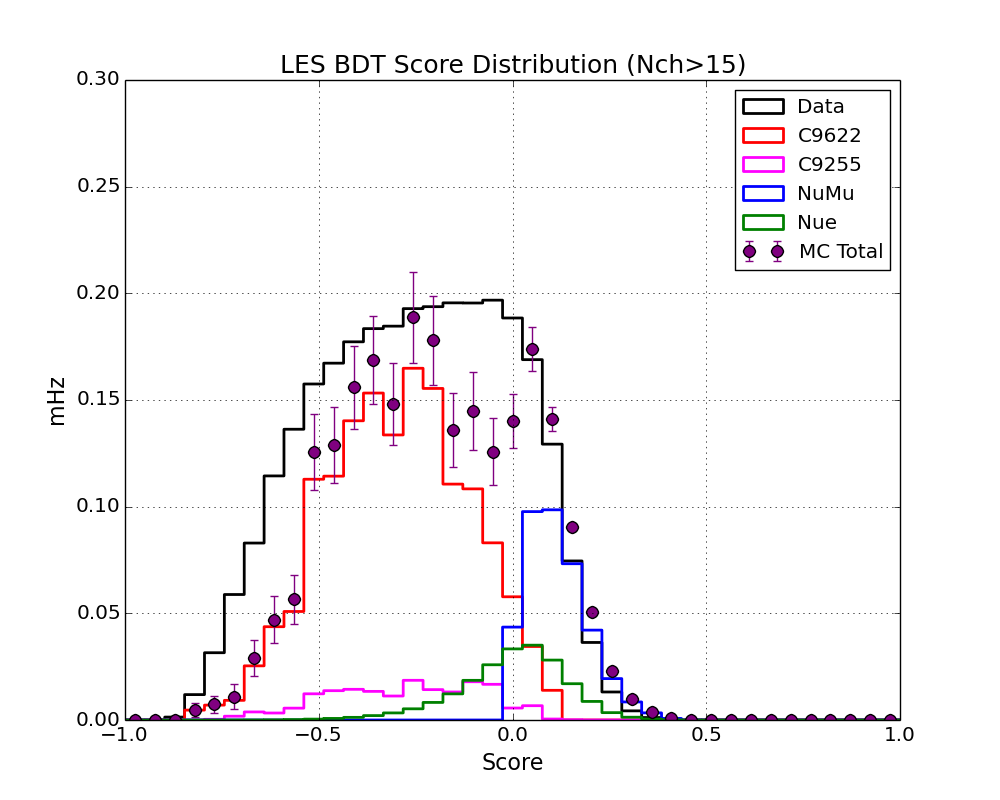
\includegraphics[width=0.5\textwidth,keepaspectratio]{plots/LES_BDTScoreDist_NormalizedRates_WC9255_And_H3AC9622_L6_NchCut_G1460.png}
  \end{center}
  \caption[Low-Energy Event Branch BDT Score Distribution]{Still unsure of what BDT related plot to show.}
  \label{fig:LESBDTDistribution}
\end{figure}

The final event sample given after the application of the BDT cuts consists of 22,040 events over a livetime of $\sim$330 days. The sample is composed mostly of atmospheric neutrinos with an estimated neutrino purity of 90$\%$. [Give median resolution here?]

\section{Analysis Method}
The search methods employed in the analysis of this data are nearly identical to those used in previous time-dependent IceCube analyses (see \cite{2008APh....29..299B} and \cite{2015arXiv150300598A}). The arrival times and directions of events within the dataset are fed to a likelihood function which is then used to perform a likelihood ratio test to compare a signal plus background hypothesis for the data to the background only hypothesis.

Construction of this likelihood function begins with the assignment of individual event probabilities that reflect the likelihood of seeing an event $i$ with arrival time $t_i$, reconstructed direction $\vec{x}_i$, and angular uncertainty $\sigma_i$ given a hypothetical source located at $\vec{x}_s$ with strength $n_s$ having a Gaussian time profile with mean time $t_0$ and width $\sigma_w$.
\begin{equation}\label{eq:EventProb}
\mathcal{P}_i(\vec{x}_i,t_i,\sigma_i|\vec{x}_s,n_s,t_0,\sigma_w) = \frac{n_s}{n_{\mathrm{tot}}} \mathcal{S}_i + \left(1-\frac{n_s}{n_{\mathrm{tot}}}\right) \mathcal{B}_i
\end{equation}
The $\mathcal{S}_i$ and $\mathcal{B}_i$ terms listed in Eq. \ref{eq:EventProb} are the signal and background probability density functions (p.d.f.) respectively. The p.d.f.s used in this search differ slightly from those in previously reported searches in that they use no reconstructed energy information. The signal p.d.f. is given by
\begin{equation}
\mathcal{S}_i(|\mathbf{x}_i-\mathbf{x}_s|,t_i,t_o,\sigma_w,\sigma_i) = S_i(|\mathbf{x}_i-\mathbf{x}_s|,\sigma_i) \cdot T_i(t_i,t_o,\sigma_w)
\end{equation}
where
\begin{equation}
S_i(|\mathbf{x}_i-\mathbf{x}_s|,\sigma_i) = \frac{\kappa}{4\pi \sinh \kappa} \exp \left(\kappa \cos |\mathbf{x}_i-\mathbf{x_s}|\right)
\end{equation}
and
\begin{equation}
T_i(t_i,t_o,\sigma_w) = \frac{1}{\sqrt{2\pi}\sigma_w} \exp \left(-\frac{(t_i-t_o)^2}{2 \sigma_w^2}\right)
\end{equation}
The spatial component of the signal p.d.f., $S_i$, features another difference with respect to previous searches (see \cite{2014ApJ...796..109A}). Due to the larger estimated error in reconstructed direction for low energy events, the Kent-Fisher distribution is used to model the probability of event-source association, and it is analogous to the Gaussian distribution normalized to the 2-sphere \citep{Fisher_Bingham}.

The background p.d.f., $\mathcal{B}_i$, is derived from the final level data set which is dominated by background. It has the following form
\begin{equation}
\mathcal{B}_i(\mathbf{x}_i,t_i) = P_{BkgDec}(\delta_i)\frac{P_{BkgAz}(\alpha_i)}{T}
\end{equation}
where $T$ is the total livetime of the search, $P_{BkgDec}(\delta_i)$ is a p.d.f. describing the event declination distribution, and $P_{BkgAz}(\alpha_i)$ is a p.d.f. describing the event distribution in detector azimuth. These p.d.f.s are generated directly from data and do not depend on any background simulation.

The likelihood function itself is simply the product sum of all individual event probabilities:
\begin{equation}\label{eq:LLH}
\mathcal{L}(\mathbf{x}_s,n_s,t_0,\sigma_w) = \prod \mathcal{P}_i(|\mathbf{x}_i-\mathbf{x}_s|,n_s,t_i,t_0,\sigma_w,\sigma_i)
\end{equation}
The ratio between the likelihood function values under the background only hypothesis ($n_s=0$) and the signal plus background hypothesis is maximized through variation of the source parameters $n_s$, $\sigma_w$, and $t_0$. The test statistic $\hat{\lambda}$ is then defined as the maximum value of the likelihood ratio:
\begin{equation}\label{eq:TS}
\hat{\lambda} = -2\log \left[\frac{\sqrt{2\pi}\hat{\sigma}_w}{T}\frac{\mathcal{L}(n_s = 0)}{\mathcal{L}(\vec{x}_s,\hat{n}_s,\hat{t}_o,\hat{\sigma}_w)} \right]
\end{equation}
with $\mathcal{L}(n_s = 0)$ corresponding to the likelihood of the null hypothesis and $\mathcal{L}(\vec{x}_s,{n}_s,\hat{t}_o,\hat{\sigma}_w)$ the likelihood of the signal plus background hypothesis with the best-fit values of the source parameters. Because this is a search for sources of finite duration over a timescale of limited duration, the number of potential short duration flares within the data set exceeds that of flares of longer duration leading to an effective trials factor. This results in a bias towards flares of shorter duration. We counteract this effect through the introduction of a marginalization term $T/\sqrt{2\pi}\hat{\sigma_w}$ in test statistic formulation which serves to penalize flares of shorter duration. More details about this term and its justification can be found in \cite{2010APh....33..175B}.

The test statistic is defined such that it will asymptotically follow a $\chi^2$ distribution with degrees of freedom corresponding to the number of fitted parameters for data consisting solely of background events. This enables the value of the maximized test statistic $\hat{\lambda}$ to be used to estimate the pre-trials p-value of the best-fit flare. Because this search attempts to look many times over the whole Northern sky, the actual significance of a given flare will need to be adjusted to account for the effective number of trials accrued during the sky scan. We use the procedure detailed in \cite{2015arXiv150300598A} that involves scrambling the event arrival times in the final dataset which also serves to scramble event right ascension. The search is performed on the randomized background data set and the p-value of the most significant flare in the search is recorded. Many iterations are performed to build a distribution of p-values which can then be compared to the p-value of the result from the real data. The fraction of background trials that result in a p-value of equal or greater significance than the observed p-value dictates the probability that the observed result is simply the consequence of a random background fluctuation. This probability is referred to as the post-trials p-value and it represents the true significance of the search result with proper trials factor correction.

In order to preserve generality, the presented search makes no use of information outside of the data set to designate source regions or time periods of interest. Instead, each point in the sky over a declination band ranging from -5$^{\circ}$ to 90$^{\circ}$ is examined. This is accomplished by discretizing the sky into separate bins and letting the location of these bins serve as the location of a hypothetical flaring source. Maximization of the likelihood is then performed at each bin to obtain a test statistic $\hat{\lambda}$ for each bin. The first iteration of this scan uses a relatively coarse 2$^{\circ}$ by 2$^{\circ}$ binning. Following completion of this first scan, a followup scan with finer 0.5$^{\circ}$ by 0.5$^{\circ}$ binning is performed over coarse bins featuring a pre-trials p-value more significant than a predefined threshold ($-\log_{10}($p-value$) > 1.75$). The result is a map of pre-trials p-values which shows the estimated significance of the best-fit flare hypothesis at each bin. The best-fit flare from the bin featuring the most significant maximized test statistic after both scans is returned as the hottest spot in the search.

\section{Results and Interpretations}
Applying the described analysis method on the unscrambled dataset yields the skymap of the pre-trials p-values shown in Figure \ref{fig:RealSkyMap}. The most significant flare is located at (RA, Dec.) = (268.75$^{\circ}$, 54.25$^{\circ}$) with a signal strength $n_s$ of 13.53 signal events and has a width $\sigma_w$ of 5.89 days with the peak occurring on MJD 56107 (2012 June 29). The pre-trials p-value for this flare is estimated at 6.68$\times 10^{-5}$. The post-trials probability of seeing such a flare from background only data is 56$\%$ indicating that this flare is entirely consistent with a background only explanation of the data.
\begin{figure}[ht]
  \begin{center}
    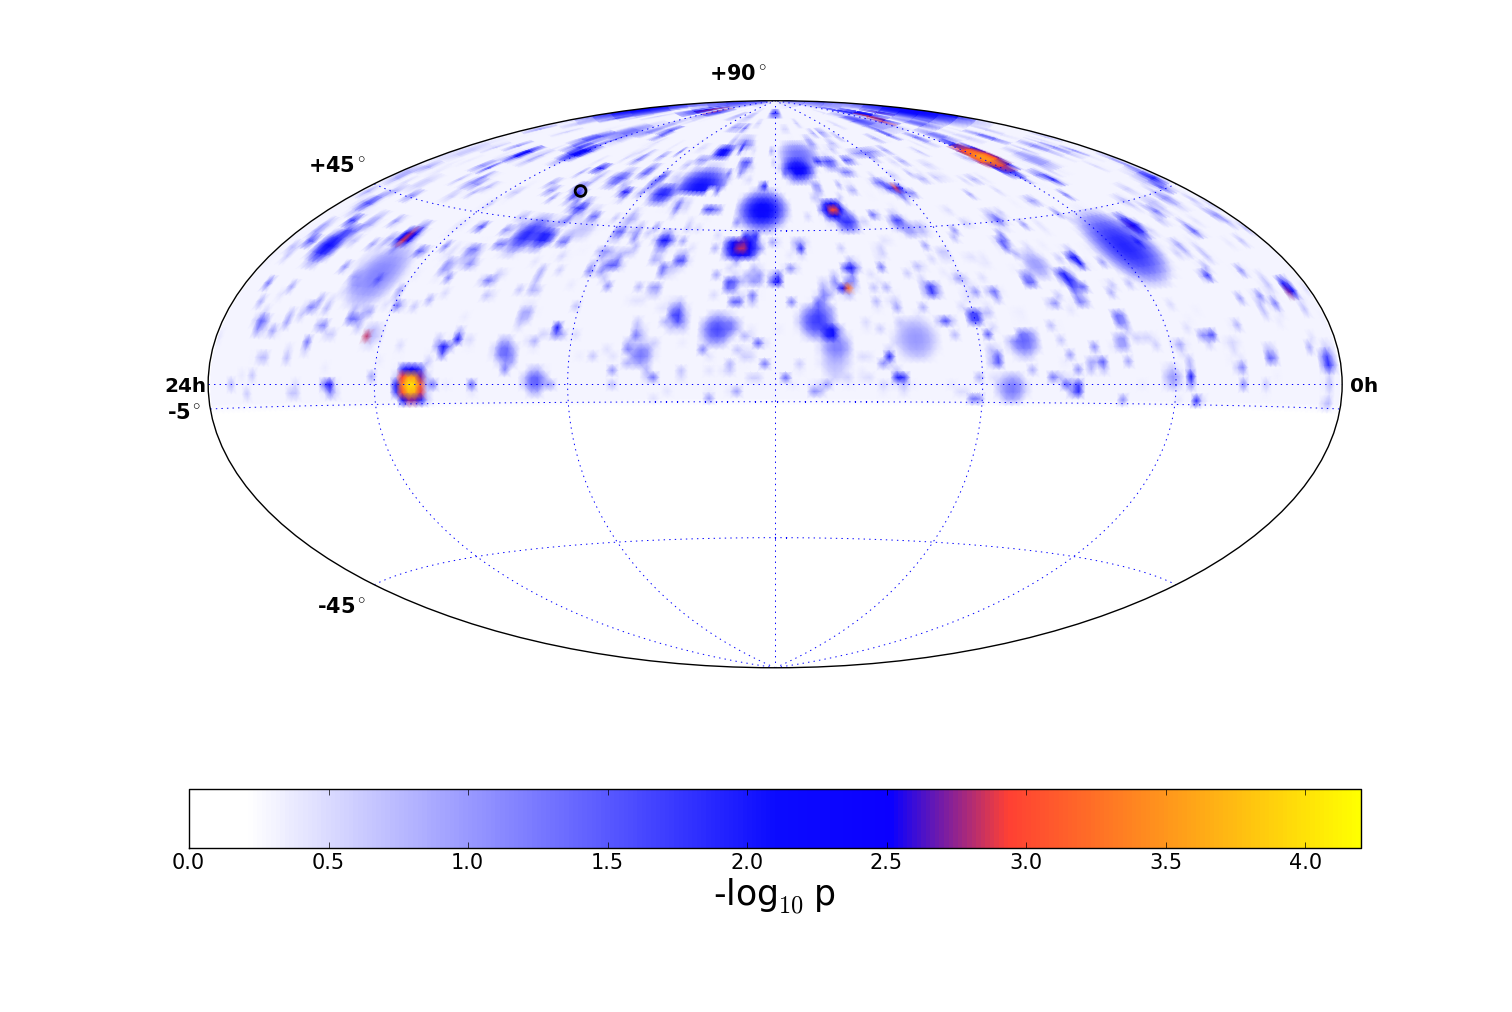
\includegraphics[width=1.0\textwidth,keepaspectratio]{plots/RealResultSkyMap.png}
  \end{center}
  \caption[Results Sky Map]{Sky map of pre-trials p-values for best fit flares per bin. The black circle identifies the location of the most significant flare found at RA = 268.75$^\circ$ and Declination = 54.25$^\circ$.}
  \label{fig:RealSkyMap}
\end{figure}
Given this null result, we can set an upper limit on the neutrino flux of any possible unobserved neutrino flare that may have occurred during the search period. Due to the focus on low-energy events in this search, we choose to examine the limit with respect to a soft-spectrum $E^{-3}$ generic flaring neutrino source with a Gaussian emission profile. An an upper limit is established through signal injections at a specified location. The background p-value distribution at the chosen location is constructed from several time scramblings of the data. Signal events are then injected with some Poisson mean value that is increased until the recovered p-values from the injections exceeds that of the median background p-value 90$\%$ of the time. This Poisson mean number of signal events is then taken as an event upper limit for the analysis method.

The upper limit for this generic flaring source for several emission timescales and choices of declination is plotted in Figure \ref{fig:GenericE3Limit}. The limit begins to rise precipitously at longer timescales as the rate of coincidental nearby background events becomes non-negligible. A limit on the time-integrated flux (GeV$^{-1} \cdot$ cm$^{-2}$) is plotted as well. This limit is obtained by folding the source spectrum with the effective area of the event selection and normalizing the flux so that the number of events produced in the detector corresponds to the calculated Poisson mean event upper limit. 

\begin{figure}[ht]
\plottwo{plots/LowEnTransient_UpperLimit_E3_G1460_Avg_DoubleY.png}{plots/LowEnTransient_FluxSensitivity_E3_G1460_MultiDec.png}
\caption[Time-integrated Flux Limit for E$^{-3}$ Source]{Upper limit (90$\%$ C.L.) for a generic E$^{-3}$ transient source as a function of flare width $\sigma_w$.The limit is given in mean number of events (left axis) as well as in time-integrated flux at a reference energy of 100 GeV (right axis).}
\label{fig:GenericE3Limit}
\end{figure}

\subsection{Choked GRB Limits}
This null result can also be used to construct limits on specific neutrino emission models such as the model for choked GRB emission by \cite{2004PhRvL..93r1101R} and \cite{2005PhRvL..95f1103A} mentioned previously (this will hereafter be referred to as RMW/AB). Unlike the hard spectra sources (e.g, E$^{-2}$) that are the typical target in IceCube searches, the neutrino flux for choked GRBs is predicted to be much softer. The spectral shape can be modeled via a doubly broken power law with spectral breaks occurring as hadronic ($E_{\nu^{(1)}}$) and radiative ($E_{\nu^{(2)}}$) cooling mechanisms become efficient respectively (see Eq. \ref{eq:chkgrb_spec}). 
\begin{equation}\label{eq:chkgrb_spec}
\frac{d\Phi_\nu}{dE}=F_\nu\left\{\begin{array}{cc}
E^{-2} & E > E_{\nu}^{(1)} \\ 
E_{\nu}^{(1)}E^{-3} & E_{\nu}^{(1)}< E < E_{\nu}^{(2)} \\ 
E_{\nu}^{(1)}E_{\nu}^{(2)}E^{-4} & E_{\nu}^{(2)}< E < E_{max}
\end{array}\right.
\end{equation}
\begin{equation}\label{eq:nuflu}
F_{\nu} = \frac{<n>_{\pi(K)}B_{\pi(K)}}{8} \cdot \frac{E_j \Gamma_b^2}{2 \pi D^2 \textrm{ln}(E_{p,max}'/ E_{p,min}')}
\end{equation}
The fluence $F_\nu$ at Earth is given by Eq. \ref{eq:nuflu} and depends upon the pion (kaon) multiplicity $<n>$, neutrino production branching ratio for pions (kaons) $B_{\pi(K)}$, minimum and maximum proton energies ($E_{p,min}', E_{p,max}'$), kinetic energy of the jet $E_j$, bulk Lorentz factor $\Gamma_b$, and lastly the distance to the source $D$. Equations \ref{eq:chkgrb_spec} and \ref{eq:nuflu} reveal that the normalization and spectral shape of the neutrino flux at Earth is highly dependent on the kinetic energy of the jet $E_j$ and the bulk lorentz factor $\Gamma_b$. We therefore choose to examine the predicted neutrino fluence in $E_j$-$\Gamma_b$ phase space. 

To ascertain which values of these parameters produce a fluence detectable through our search method, an event upper limit is first determined via the injection of signal events following a spectrum set by the value of $E_j$ and $\Gamma_b$ (the same process used to generate an event upper limit for the generic $E^{-3}$ scenario). This event upper limit then is then combined with the effective area of the event selection to determine the neutrino fluence necessary for detection. For a given choice of $E_j$ and $\Gamma_b$ this sets a limit on the distance at which the source would still be visible to the search; we define this distance $D_{vis}$ as the visibility distance.

When combined with the area of sky examined by the search $\Omega_{A}$, this visibility distance in turn defines a parameter dependent volume $V_A$ over which the search method monitors where $V_A=\frac{1}{3}\Omega_{A}D_{vis}^{3}$. The monitored volume $V_A$ corresponds to the volume in which a choked GRB event would have been detected by the search method with 90$\%$ confidence (assuming jet alignment). If the observation period of the search is considered, this monitored volume can be converted into a limit on the volumetric rate of choked GRB events as a function of $E_j$ and $\Gamma_b$. This requires two assumptions to be made however: 1) The jets of any choked GRB event in this volume are aligned with Earth and 2) The nearby universe is homogeneous with respect to CC SNe production. The rate limit is then given by
\begin{equation}\label{eq:ratelimit}
R = \left(\frac{U.L.(0|\mu)}{\tau \cdot V_A}\right)
\end{equation}
where $\tau$ is the livetime of the search, $V_A$ is the monitored volume previously defined, and $U.L.(0|\mu)$ is the null observation upper limit on the number of choked GRBs that occurred in our monitored volume with background expectation of $\mu$. Many iterations of the search performed with only background data determined the probability of a background false positive rate to be very small ($\leq 10^{-3}$). We therefore take $\mu\approx0$ leading to a Neyman upper limit of 2.3 from the null observation.
\begin{figure}[ht]
  \begin{center}
    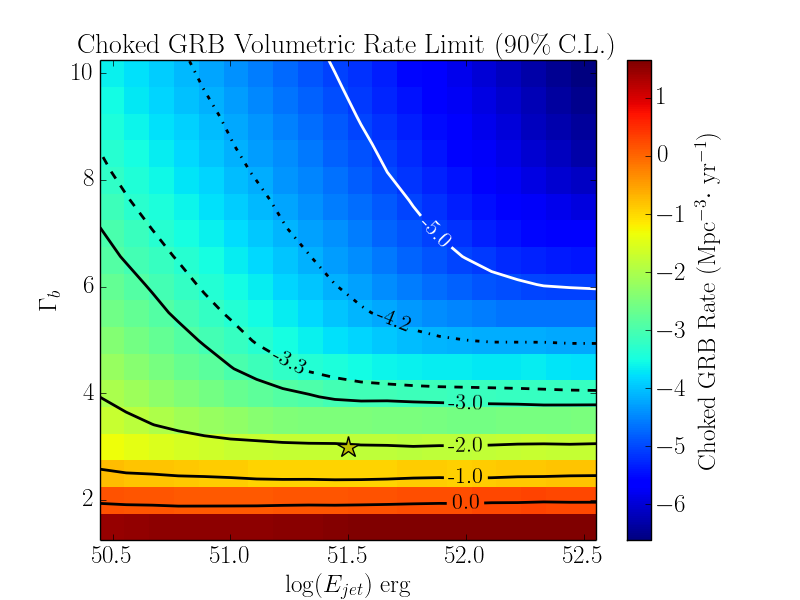
\includegraphics[width=0.8\textwidth,keepaspectratio]{plots/RateLimit_2DHisto_wContours_SysAdj.png}
  \end{center}
  \caption[Choked GRB Volumetric Rate Limit]{Histogram of the rate limit on choked GRBs in the nearby universe. The bin for canonical values of the neutrino emission model is marked by the star. The dashed line contour gives the rate of core-collapse supernovae within 10 Mpc as measured by \cite{2011PhRvD..83l3008K}. The dot-dashed line is the volumetric rate extracted from a large survey of SNe in the local universe \citep{2011MNRAS.412.1419L}}
  \label{fig:VolumetricRateLimit}
\end{figure}

The volumetric rate limit for a range of values of jet kinetic energy and bulk Lorentz factor is plotted in Figure \ref{fig:VolumetricRateLimit}. In addition to the calculated volumetric rate limits, two separate measurements of the nearby CC SNe are also plotted to provide context to the limits. Choked GRB events harboring particularly energetic jet parameters should be visible to the search method. If one compares the limits for the canonical model parameter values ($\Gamma_b = 3$, $E_j = 10^{51.5}$ erg) to the CC SNe rates, it is clear that the search method is not very sensitive to large regions of the model parameter space in its current state. The capabilities of future iterations of this type of search should be considerably improved as both the event selection and analysis methods are further refined.	
\section{Conclusions}
The search described in this paper examined a newly developed data set consisting of 30-300 GeV muon neutrinos. No evidence for transient astrophysical neutrino sources was found in the data leading to the construction of upper limits on the neutrino fluence of potential sources within the observation period. These limits serve to complement existing IceCube searches by examining a relatively unexplored energy range. Furthermore, the sensitivity of this method will only improve as the event selection and search techniques are further optimized for muon neutrino events at sub-TeV energies.



\acknowledgments
We acknowledge support from the following agencies: U.S. National Science 
Foundation-Office of Polar Programs, U.S. National Science Foundation-Physics
Division, University of Wisconsin Alumni Research Foundation, the Grid
Laboratory Of Wisconsin (GLOW) grid infrastructure at the University of
Wisconsin - Madison, the Open Science Grid (OSG) grid infrastructure; U.S.
Department of Energy, and National Energy Research Scientific Computing Center, 
the Louisiana Optical Network Initiative (LONI) grid computing resources;
Natural Sciences and Engineering Research Council of Canada, WestGrid and
Compute/Calcul Canada; Swedish Research Council, Swedish Polar Research
Secretariat, Swedish National Infrastructure for Comput ing (SNIC), and Knut
and Alice Wallenberg Foundation, Sweden; German Ministry for Education and
Research (BMBF), Deutsche Forschungsgemeinschaft (DFG), Helmholtz Alliance for
Astroparticle Physics (HAP), Research Department of Plasmas with Complex 
Interactions (Bochum), Germany; Fund for Scientific Research (FNRS-FWO), FWO
Odysseus programme, Flanders Institute to encourage scientific and
technological research in industry (IWT), Belgian Federal Science Policy Office
(Belspo); University of Oxford, United Kingdom; Marsden Fund, New Zealand;
Australian Research Council; Japan Society for Promotion of Science (JSPS); the
Swiss National Science Foundation (SNSF), Switzerland; National Research
Foundation of Korea (NRF); Danish National Research Foundation, Denmark (DNRF). 


\bibliography{IceCube_2012_LowEnTransient}{}

\clearpage

%% Use the figure environment and \plotone or \plottwo to include
%% figures and captions in your electronic submission.
%% To embed the sample graphics in
%% the file, uncomment the \plotone, \plottwo, and
%% \includegraphics commands
%%
%% If you need a layout that cannot be achieved with \plotone or
%% \plottwo, you can invoke the graphicx package directly with the
%% \includegraphics command or use \plotfiddle. For more information,
%% please see the tutorial on "Using Electronic Art with AASTeX" in the
%% documentation section at the AASTeX Web site, http://aastex.aas.org/
%%
%% The examples below also include sample markup for submission of
%% supplemental electronic materials. As always, be sure to check
%% the instructions to authors for the journal you are submitting to
%% for specific submissions guidelines as they vary from
%% journal to journal.

%% This example uses \plotone to include an EPS file scaled to
%% 80% of its natural size with \epsscale. Its caption
%% has been written to indicate that additional figure parts will be
%% available in the electronic journal.

%\begin{figure}
%\epsscale{.80}
%\plotone{f1.eps}
%\caption{Derived spectra for 3C138 \citep[see][]{heiles03}. Plots for all %sources are available
%in the electronic edition of {\it The Astrophysical Journal}.\label{fig1}}
%\end{figure}

\clearpage

%% Here we use \plottwo to present two versions of the same figure,
%% one in black and white for print the other in RGB color
%% for online presentation. Note that the caption indicates
%% that a color version of the figure will be available online.
%%

%\begin{figure}
%\plottwo{f2.eps}{f2_color.eps}
%\caption{A panel taken from Figure 2 of \citet{rudnick03}. 
%See the electronic edition of the Journal for a color version 
%of this figure.\label{fig2}}
%\end{figure}

%% This figure uses \includegraphics to scale and rotate the still frame
%% for an mpeg animation.

%\begin{figure}
%\includegraphics[angle=90,scale=.50]{f3.eps}
%\caption{Animation still frame taken from \citet{kim03}.
%This figure is also available as an mpeg
%animation in the electronic edition of the
%{\it Astrophysical Journal}.}
%\end{figure}

%% If you are not including electonic art with your submission, you may
%% mark up your captions using the \figcaption command. See the
%% User Guide for details.
%%
%% No more than seven \figcaption commands are allowed per page,
%% so if you have more than seven captions, insert a \clearpage
%% after every seventh one.

%% Tables should be submitted one per page, so put a \clearpage before
%% each one.

%% Two options are available to the author for producing tables:  the
%% deluxetable environment provided by the AASTeX package or the LaTeX
%% table environment.  Use of deluxetable is preferred.
%%

%% Three table samples follow, two marked up in the deluxetable environment,
%% one marked up as a LaTeX table.

%% In this first example, note that the \tabletypesize{}
%% command has been used to reduce the font size of the table.
%% We also use the \rotate command to rotate the table to
%% landscape orientation since it is very wide even at the
%% reduced font size.
%%
%% Note also that the \label command needs to be placed
%% inside the \tablecaption.

%% This table also includes a table comment indicating that the full
%% version will be available in machine-readable format in the electronic
%% edition.

\clearpage


\end{document}